% slides completed June 22, 2008
% for Krakow conference


\documentclass{beamer}
  \usetheme{Boadilla}
% \usetheme{Madrid}
% \usetheme{Montpellier}
% \usetheme{Warsaw}
% \usetheme{default}
 
% \usecolortheme{crane}
 % \beamertemplatesolidbackgroundcolor{craneorange!25}
 
% math notation shortcuts

\newcommand{\ar}{\rightarrow}
\newcommand{\ds}{\displaystyle}
\newcommand{\ab}{\alpha\beta}
\newcommand{\ba}{\beta\alpha}


\newcommand{\diam}{\mbox{\rm diam\,}}
\newcommand{\vol}{\mbox{\rm vol\,}}

\newcommand{\Ma}{M_{\alpha}}
\newcommand{\cd}{\mbox{\rm cd}(M,\F)}
\newcommand{\codim}{\mbox{\rm codim}}

\newcommand{\hpa}{\hat{\phi}_{\alpha}}

\newcommand{\ord}{\mbox{\rm ord}_{\F}(M)}

\newcommand{\simF}{~ {\simeq}_{\F} ~}

\newcommand{\vt}{{\vec{\theta}}}

\newcommand{\EF}{E({\F})}
\newcommand{\EG}{E({\cG})}

\newcommand{\sop}{{\bf Proof:} }
\newcommand{\eop}{\;\;\;  \Box}
 
% bold letters

\newcommand{\C}{{\mathbf C}}
\newcommand{\K}{{\mathbf K}}
\newcommand{\Q}{{\mathbf Q}}
\newcommand{\R}{{\mathbf R}}
\newcommand{\T}{{\mathbf T}}
\newcommand{\X}{{\mathbf X}}
\newcommand{\Z}{{\mathbf Z}}


% foliations

  
\newcommand{\F}{{\mathcal F}}
  
\newcommand{\Fa}{{\mathcal F}_{\alpha}}
\newcommand{\TF}{T{\mathcal F}}

\newcommand{\wF}{{\widehat{\F}}}

\newcommand{\wtF}{{\widetilde{\mathcal F}}}

% leaf notations

\newcommand{\wL}{\widetilde{L}}

% holonomy notations

\newcommand{\G}{\Gamma}

\newcommand{\GF}{{\mathcal G}_{\F}}
\newcommand{\Gh}{{\mathcal G}^h_{\F}}

\newcommand{\wh}{\widetilde{\bf h}}

\newcommand{\HF}{{\mathcal H}_{\F}}
\newcommand{\ZF}{{\mathcal Z}_{\F}}

\newcommand{\hab}{{\bf h}_{\alpha \beta}}
\newcommand{\hba}{{\bf h}_{\beta \alpha}}
\newcommand{\whab}{\widetilde{\bf h}_{\alpha \beta}}
\newcommand{\whba}{\widetilde{\bf h}_{\beta \alpha}}

\newcommand{\hp}{{\mathcal H}_{\phi}}
\newcommand{\h}{h_{g}({\mathcal F})}

% transversals

\newcommand{\cTa}{{\mathcal T}_{\alpha}}
\newcommand{\cTb}{{\mathcal T}_{\beta}}
\newcommand{\cTab}{{\mathcal T}_{\alpha \beta}}
\newcommand{\cTba}{{\mathcal T}_{\beta \alpha}}
\newcommand{\wcT}{\widetilde{\mathcal T}}
\newcommand{\wcTa}{\widetilde{\mathcal T}_{\alpha}}
\newcommand{\wcTb}{\widetilde{\mathcal T}_{\beta}}
\newcommand{\wcTab}{\widetilde{\mathcal T}_{\alpha \beta}}
\newcommand{\wcTba}{\widetilde{\mathcal T}_{\beta \alpha}}



% plaques 


\newcommand{\cPa}{{\mathcal P}_{\alpha}}
\newcommand{\cPb}{{\mathcal P}_{\beta}}
\newcommand{\wcP}{\widetilde{\mathcal P}}
\newcommand{\wcPa}{\widetilde{\mathcal P}_{\alpha}}
\newcommand{\wcPb}{\widetilde{\mathcal P}_{\beta}}


% differential operators

\newcommand{\DF}{{\mathcal D}_{\mathcal F}}
\newcommand{\DL}{{\mathcal D}_{L}}
\newcommand{\Da}{{\mathcal D}_{\alpha}}
\newcommand{\Dfa}{{\mathcal D}_{{\mathcal F}_{\alpha}}}
\newcommand{\Dx}{{\mathcal D}_x}
\newcommand{\Dy}{{\mathcal D}_y}
\newcommand{\Dz}{{\mathcal D}_z}

\newcommand{\spF}{\sigma({\mathcal D}_{\mathcal F})}
\newcommand{\spL}{\sigma({\mathcal D}_L)}
\newcommand{\sppF}{\sigma_{pp}({\mathcal D}_{\mathcal F})}
\newcommand{\sppL}{\sigma_{pp}({\mathcal D}_L)}


% vector bundles

\newcommand{\CE}{C^{\infty}({\bf E})}
\newcommand{\Ca}{{\mathbb C}_{\alpha}}
\newcommand{\EL}{{\bf E}_L}
\newcommand{\Ea}{{\bf E}_{\alpha}}
\newcommand{\E}{E_{\F}}


\newcommand{\whQe}{{\widehat{Q}^{\epsilon_0}}}
\newcommand{\wtQe}{{\widetilde{Q}^{\epsilon_0}}}

% metrics


\newcommand{\dF}{d_{\F}}
\newcommand{\dG}{d_{\Gh}}
\newcommand{\dT}{d_{\cT}}
 
\newcommand{\dwtF}{{d_{\widetilde{\F}}}}

\newcommand{\whdF}{{\widehat{d}_{\F}}}

\newcommand{\wtdF}{{\widetilde{d}_{\F}}}

% various sets

 \newcommand{\D}{{{\mathbb D}^q}}
\newcommand{\Dr}{{{\ mathbb D}_r^q}}

% epsilons

\newcommand{\ez}{{\epsilon_0}}
\newcommand{\eone}{{\epsilon_1}}
\newcommand{\etwo}{{\epsilon_2}}
\newcommand{\ethree}{{\epsilon_3}}
\newcommand{\estar}{{\epsilon_*}}
 
 
\newcommand{\eF}{\epsilon_{\F}}


% bold maps

\newcommand{\hf}{{\bf f}}
\newcommand{\hh}{{\bf h}}
\newcommand{\hH}{{\bf H}}
\newcommand{\hk}{{\bf k}}
\newcommand{\m}{{\bf m}}
\newcommand{\hg}{{\bf g}}
\newcommand{\bO}{{\bf O}}
\newcommand{\bSO}{{\bf SO}}


 % math blackboard bolds

  
  
\newcommand{\mA}{{\mathbb A}}
\newcommand{\mB}{{\mathbb B}}
\newcommand{\mC}{{\mathbb C}}
\newcommand{\mD}{{\mathbb D}}
\newcommand{\mE}{{\mathbb E}}
\newcommand{\mF}{{\mathbb F}}
\newcommand{\mG}{{\mathbb G}}
\newcommand{\mH}{{\mathbb H}}
\newcommand{\mI}{{\mathbb I}}
\newcommand{\mJ}{{\mathbb J}}
\newcommand{\mK}{{\mathbb K}}
\newcommand{\mL}{{\mathbb L}}
\newcommand{\mM}{{\mathbb M}}
\newcommand{\mN}{{\mathbb N}}
\newcommand{\mO}{{\mathbb O}}
\newcommand{\mP}{{\mathbb P}}
\newcommand{\mQ}{{\mathbb Q}}
\newcommand{\mR}{{\mathbb R}}
\newcommand{\mS}{{\mathbb S}}
\newcommand{\mT}{{\mathbb T}}
\newcommand{\mU}{{\mathbb U}}
\newcommand{\mV}{{\mathbb V}}
\newcommand{\mW}{{\mathbb W}}
\newcommand{\mX}{{\mathbb X}}
\newcommand{\mY}{{\mathbb Y}}
\newcommand{\mZ}{{\mathbb Z}}

% cal script letters

\newcommand{\cA}{{\mathcal A}}
\newcommand{\cB}{{\mathcal B}}
\newcommand{\cC}{{\mathcal C}}
\newcommand{\cD}{{\mathcal D}}
\newcommand{\cE}{{\mathcal E}}
\newcommand{\cF}{{\mathcal F}}
\newcommand{\cG}{{\mathcal G}}
\newcommand{\cH}{{\mathcal H}}
\newcommand{\cI}{{\mathcal I}}
\newcommand{\cJ}{{\mathcal J}}
\newcommand{\cK}{{\mathcal K}}
\newcommand{\cL}{{\mathcal L}}
\newcommand{\cM}{{\mathcal M}}
\newcommand{\cN}{{\mathcal N}}
\newcommand{\cO}{{\mathcal O}}
\newcommand{\cP}{{\mathcal P}}
\newcommand{\cQ}{{\mathcal Q}}
\newcommand{\cR}{{\mathcal R}}
\newcommand{\cS}{{\mathcal S}}
\newcommand{\cT}{{\mathcal T}}
\newcommand{\cU}{{\mathcal U}}
\newcommand{\cV}{{\mathcal V}}
\newcommand{\cW}{{\mathcal W}}
\newcommand{\cX}{{\mathcal X}}
\newcommand{\cY}{{\mathcal Y}}
\newcommand{\cZ}{{\mathcal Z}}



% widetilde uppercase letters

\newcommand{\wtA}{{\widetilde A}}
\newcommand{\wtB}{{\widetilde B}}
\newcommand{\wtC}{{\widetilde C}}
\newcommand{\wtD}{{\widetilde D}}
\newcommand{\wtE}{{\widetilde E}}
\newcommand{\wtG}{{\widetilde G}}
\newcommand{\wtH}{{\widetilde H}}
\newcommand{\wtI}{{\widetilde I}}
\newcommand{\wtJ}{{\widetilde J}}
\newcommand{\wtK}{{\widetilde K}}
\newcommand{\wtL}{{\widetilde L}}
\newcommand{\wtM}{{\widetilde M}}
\newcommand{\wtN}{{\widetilde N}}
\newcommand{\wtO}{{\widetilde O}}
\newcommand{\wtP}{{\widetilde P}}
\newcommand{\wtQ}{{\widetilde Q}}
\newcommand{\wtR}{{\widetilde R}}
\newcommand{\wtS}{{\widetilde S}}
\newcommand{\wtT}{{\widetilde T}}
\newcommand{\wtU}{{\widetilde U}}
\newcommand{\wtV}{{\widetilde V}}
\newcommand{\wtW}{{\widetilde W}}
\newcommand{\wtX}{{\widetilde X}}
\newcommand{\wtY}{{\widetilde Y}}
\newcommand{\wtZ}{{\widetilde Z}}
\newcommand{\wtDel}{{\widetilde{\Delta}}}

% widetilde lowercase letters

\newcommand{\wtd}{{\widetilde{d}}}
\newcommand{\wtg}{{\widetilde{g}}}
\newcommand{\wtx}{{\widetilde{x}}}
\newcommand{\wtz}{{\widetilde{z}}}
\newcommand{\wty}{{\widetilde{y}}}
\newcommand{\wtpi}{{\widetilde{\pi}}}
\newcommand{\wtnu}{{\widetilde{\nu}}}
\newcommand{\wtiota}{{\widetilde{\iota}}}

% widehat uppercase letters

\newcommand{\whA}{{\widehat A}}
\newcommand{\whB}{{\widehat B}}
\newcommand{\whC}{{\widehat C}}
\newcommand{\whD}{{\widehat D}}
\newcommand{\whE}{{\widehat E}}
\newcommand{\whF}{{\widehat{F}}}
\newcommand{\whG}{{\widehat G}}
\newcommand{\whH}{{\widehat H}}
\newcommand{\whI}{{\widehat I}}
\newcommand{\whJ}{{\widehat J}}
\newcommand{\whK}{{\widehat K}}
\newcommand{\whL}{{\widehat L}}
\newcommand{\whM}{{\widehat M}}
\newcommand{\whN}{{\widehat N}}
\newcommand{\whO}{{\widehat O}}
\newcommand{\whP}{{\widehat P}}
\newcommand{\whQ}{{\widehat{Q}}}
\newcommand{\whR}{{\widehat R}}
\newcommand{\whS}{{\widehat S}}
\newcommand{\whT}{{\widehat T}}
\newcommand{\whU}{{\widehat U}}
\newcommand{\whV}{{\widehat V}}
\newcommand{\whW}{{\widehat W}}
\newcommand{\whX}{{\widehat{X}}}
\newcommand{\whY}{{\widehat Y}}
\newcommand{\whZ}{{\widehat{Z}}}
 

% widehat lowercase letters

\newcommand{\whd}{{\widehat{d}}}
\newcommand{\whg}{{\widehat{g}}}
\newcommand{\whr}{{\widehat{r}}}
\newcommand{\whx}{{\widehat{x}}}
\newcommand{\why}{{\widehat{y}}}
\newcommand{\whz}{{\widehat{z}}}
\newcommand{\whpi}{{\widehat{\pi}}}
\newcommand{\whnu}{{\widehat{\nu}}}

 
 % category notations
 
\def\subtrans{\mathbin{\cap{\mkern-9mu}\mid}\,\,}
\newcommand{\catF}{\cat_{\F}(M)}
\newcommand{\cat}{\mbox{\rm cat}}
\newcommand{\catt}{\cat_{\subtrans}}
\newcommand{\catts}{\cat^{\subtrans}_s}
\newcommand{\trans}
{
\begin{picture}(4,1)
\put(1,1){\makebox(0,0){$\cap$}}
\put(.6,1){\makebox(0,0){$\mid$}}
\end{picture}
}

 
 
 
 
\date[July 7-11, 2008]
 {VIII International Colloquium on Differential Geometry \\
Santiago de Compostela, 7-11 July 2008}

  
\title[Cohomology of Foliations]{Dynamics and Cohomology of Foliations}
 
 
\author{Steven Hurder}
 
\institute[UIC] {University of Illinois at Chicago\\www.math.uic.edu/$\sim$hurder}

 

\begin{document}

\frame{\titlepage} % # 1

% \section[Outline]{}
% \frame{\tableofcontents}

\section{Introduction}
 
  
 
\frame % 3
{
  \frametitle{Definition of foliation}
 
  A foliation $\mathcal F$ of dimension $p$ on a manifold $M^m$ is a 
 decomposition  into ``uniform layers'' -- the leaves -- which are immersed submanifolds of codimension $q$:  there is an open covering of $M$ by   coordinate charts 
so that the leaves are mapped into linear planes of dimension $p$, and the transition function preserves these planes.
\begin{center}
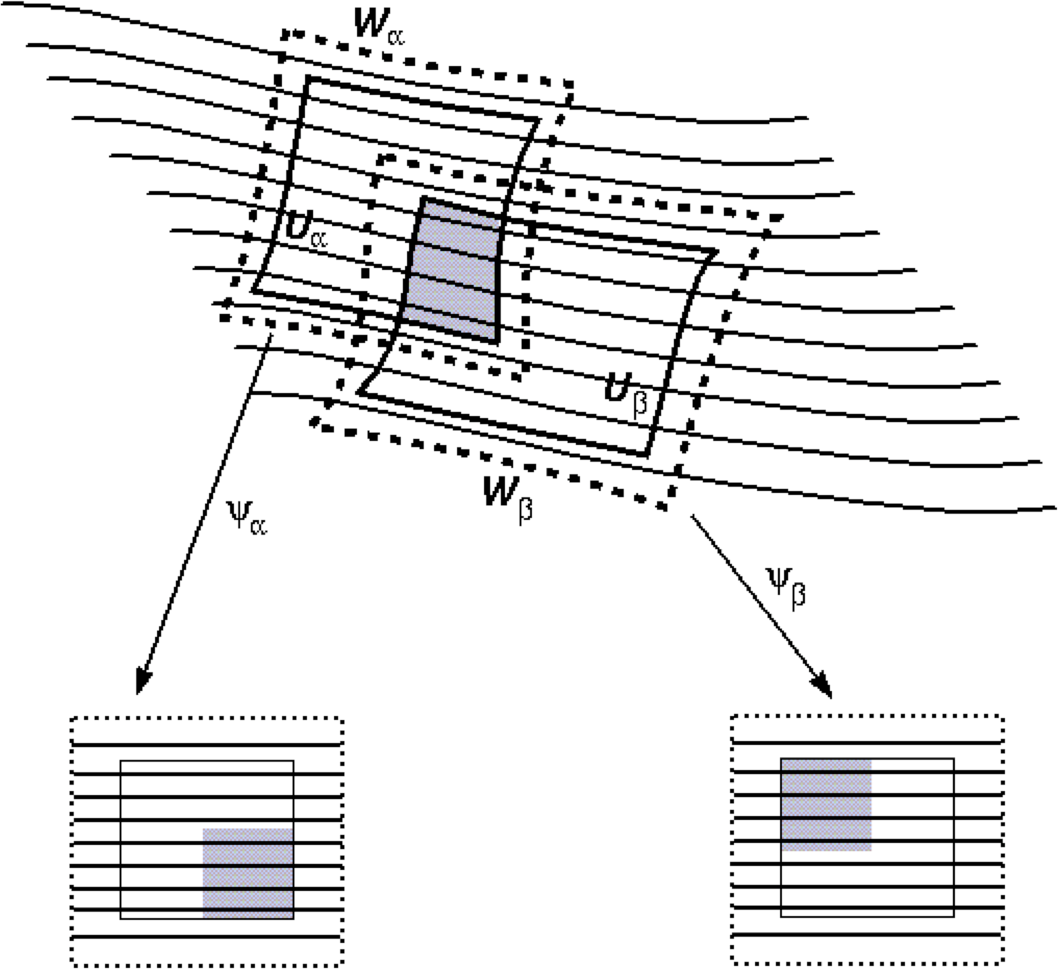
\includegraphics[width=0.35\textwidth]{pix/chart.pdf}
\end{center}
 
 \vfill   

}


\frame % 4
{
  \frametitle{Fundamental problems}
 
  
 {\bf Problem:}      ``Classify'' the foliations on a given manifold $M$
  
  \bigskip
  \pause
Two classification schemes have been developed since 1970:

 using either ``homotopy'' or ``dynamics''.
 
\medskip

 {\bf Question:}   
How are the cohomology invariants of a foliation  related to its dynamical behavior?
 
    
\vfill

}


 
\frame %  
{
  \frametitle{Integrable homotopy equivalence}

 
    Let $q$ denote the codimension of the foliation $\F$.
    \medskip
    
    $q = m -p$ where $p$ is the leaf dimension, $m = \dim M$
    \medskip
    
    Assume throughout that $\F$ is transversally $C^r$ for $r \geq 2$.
 
\bigskip
 \pause
 
 {\bf Definition:} 
 Two foliations $\F_0$ and $\F_1$ of codimension $q$ on  $M$ are \emph{integrably homotopic} if there exists a foliation $\F$ of codimension $q$ on $M \times \mR$ which is transverse to the slices $M \times \{t\} \subset M \times \mR$ for $t = 0, 1$, such that the restrictions $\F | M \times \{t\} = \F_t$ for $t = 0, 1$.

\bigskip

 Integrable homotopy is a fairly weak notion of equivalence. For example, if $M$ is an open contractible manifold then any two foliations $\F_0$ and $\F_1$ on $M$ are integrably homotopic.
 
 \vfill
 
}

 
\frame % 
{
  \frametitle{Classifying  spaces:}

   
   $B\Gamma_q$ denotes the   ``classifying space''  of   codimension-$q$ foliations introduced by Andr\'{e}  Haefliger  in 1970. 
   \medskip
   
There is a natural map $\nu \colon B\Gamma_q \to BO_q$.
   

 \medskip
 \pause

   {\bf Theorem:} (Haefliger [1970]) Each   foliation  $\F$ on $M$ of codimension $q$ determines a well-defined map $h_{\F} \colon M \to B\Gamma_q$ whose homotopy class in uniquely defined by $\F$, and depends only upon the integrable homotopy class of $\F$.
    The composition $\nu \circ h_{\F} \colon M \to BO_q$ classifies the normal bundle $Q \to M$ of $\F$.
 
 \medskip
 \pause
 
  {\bf Theorem:} (Thurston [1975]) Let $M$ be a closed manifold. A map  
  $h \colon M \to B\Gamma_q \times BO_p$ for which the composition 
  $$(\nu \times Id) \circ h \colon M \to BO_q \times BO_p \to BO_m$$ 
  classifies the tangent bundle $TM$, determines an integrable homotopy class of  
   a codimension-$q$ foliation $\F_h$ on $M$.
 
 
 \vfill
 
}
 


\frame % 
{
  \frametitle{Primary characteristic classes}

The Pontrjagin classes of the  normal bundle $Q \to M$ factor through the map:
  
\begin{center}
\begin{picture}(200,60)\label{eqn-normal}
\put(40,00){$M$}
\put(120,00){$BO_q$}
\put(70,03){\vector(1,0){35}}
\put(85,10){$h_Q$}


\put(120,50){$B\Gamma_q$}
\put(125,40){\vector(0,-1){20}}
\put(130,30){$\nu$}

\put(70,20){\vector(3,2){35}}
\put(65,38){$h_{\F}$}

\end{picture}
\end{center}
 
 \pause
 
 {\bf Theorem:} (Bott [1970])  
 \begin{center}
 $h_Q^* \colon H^{\ell}(BO_q ; \mR) \to H^{\ell}(M ; \mR)$ is trivial for $\ell > 2q$.
 \end{center}
 
 \medskip 
 \pause
 
  {\bf Theorem:} (Bott-Heitsch [1972])  
   \begin{center}
$h_Q^* \colon H^{\ell}(BO_q ; \mZ) \to H^{\ell}(M ; \mZ)$ is injective for all $\ell$.
 \end{center}
 
   
 \vfill
 
}

       

\frame %  
{
  \frametitle{Secondary classes}
   
   
  {\bf Theorem:} (Godbillon-Vey [1971])  For  $q \geq 1$, the Godbillon-Vey class 
 $GV(\F) = \Delta(h_1c_1^q) \in H^{2q+1}(M; \mR)$ is an integrable homotopy invariant.
 
   
    \pause
\begin{center}
 $WO_q \cong \Lambda(h_1, h_3, \ldots, h_{q/2}) \otimes \mR[c_1, c_2, \ldots , c_q] ~, ~ d_W h_i = c_i , d_W c_i = 0$
 \end{center}
     
   {\bf Theorem:} (Bott-Haefliger, Gelfand-Fuks, Kamber-Tondeur [1972]) For  $q \geq 1$, there is a non-trivial space of secondary invariants $H^*(WO_q)$ and functorial  characteristic map 
    whose image contains the Godbillon-Vey class
\begin{center}
\begin{picture}(180,80)
\put(95,60){$H^*(B\Gamma_q ; \mR) $}
\put(115,50){\vector(0,-1){17}}
\put(50,33){\vector(3,2){36}}
\put(70,23){\vector(1,0){25}}
\put(120,40){$h_{\F}^*$}
\put(52,50){$\tilde{\Delta}$}
\put(80,28){$\Delta_{\F}$}
\put(10,20){$H^*(WO_q)$}
\put(100,20){$H^*(M; \mR)$}
\end{picture}
\end{center}

The study of the images of the maps $\Delta_{\F}$  has been the principle source of information about the (non-trivial) homotopy type of ~ $B\G_q$.
 \vfill
 
}


\frame % 6
{
  \frametitle{Homotopy chaos}


 

   {\bf Theorem:} (Bott--Heitsch [1972]) $B\Gamma^r_q$  does not have finite topological type for $q\geq 2$.
   
   \medskip
   \pause
 
 {\bf Theorem:} (Thurston [1972]) $\pi_3(B\Gamma^r_1)$ surjects onto $\mR$. 
   
   \medskip
   \pause
 
 {\bf Theorem:} (Heitsch [1978]) There are continuous families of foliations with non-trivial variations of their secondary classes for $q \geq 3$. 
    
 
   \medskip
   \pause
  
 {\bf Theorem:} (Rasmussen [1980]) There are continuous families of foliations with non-trivial variations of their secondary classes for $q = 2$.  
   
   \medskip
   \pause

 {\bf Corollary:} $B\Gamma^r_q$  has uncountable topological type for all $q \geq 1$.
  
  \medskip
   \pause
 

   {\bf Theorem:} (Hurder [1980]) For $q \geq 2$, $\pi_{n}(B\Gamma^r_q) \to \mR^{k_n} \to 0$  where $k_{2q+1} \ne 0$,   
and in general, $k_n$ has a subsequence $k_{n_{\ell}} \to \infty$

 
 \medskip
 \pause
 
 
 Secondary  classes   measure some     uncountable aspect    of  foliation geometry. 
 
 \vfill
 
}


 
\frame
{

  \frametitle{$C^{2}$ is essential}

In contrast, Takashi Tsuboi proved the following amazing result:
\medskip

{\bf Theorem:} (Tsuboi [1989]) The classifying map of the normal bundle $\nu \colon  B\Gamma^1_q \to BO(q)$
for    foliations of transverse differentiability class $C^1$  is a homotopy equivalence.

\medskip
 

The proof  is a technical tour-de-force, using Mather-Thurston type techniques for the study of $B\G$.
 
 \bigskip
 
 \pause
 
 When the $C^1$ and $C^2$ situations are radically different, one asks if there is some aspects of dynamical systems involved? (There are other reasons to ask this question, too.)
 
\vfill



}


 
\frame
{

  \frametitle{Foliation dynamics}

\begin{itemize}

 

\item
A continuous dynamical system on a compact manifold $M$ is a flow $\varphi \colon M \times \mR \to M$, where the orbit $L_x = \{\varphi_t(x) = \varphi(x,t) \mid t \in \mR\}$ is thought of as the time trajectory of the point $x \in M$.  The trajectories of the points of $M$ are necessarily points, circles or lines immersed in $M$, and the study of their aggregate and statistical behavior is the subject of ergodic theory for flows.

 \bigskip
 

\item
In foliation dynamics, we replace the concept of time-ordered trajectories with multi-dimensional futures for points. The study of the dynamics of $\F$  asks for properties of the    aggregate and statistical behavior of the collection of its leaves.

\end{itemize}
\bigskip


\vfill

}


   
  

\frame
{

  \frametitle{Pseudogroups \& Groupoids}
  
  

Every foliation admits a discrete model by choosing a section $\cT \subset M$, an embedded submanifold of dimension $q$ which intersects each leaf of $\F$ at least once, and always transversally.  The holonomy of $\F$ yields a compactly generated pseudogroup $\cG_{\F}$ acting on $\cT$.

\bigskip

 
 {\bf Definition:}
A     pseudogroup of transformations $\cG$ of $\cT$ is \emph{compactly generated}     if there is 
\begin{itemize}
\item   a relatively compact open subset $\cT_0 \subset \cT$ meeting all leaves of $\F$
\item  a finite set $\G = \{g_1, \ldots , g_k\} \subset    \cG$  such that $\langle \G \rangle =  \cG | \cT_0$; 
\item   $g_i \colon D({g_i}) \to R({g_i})$ is the restriction of  $\widetilde{g}_i \in   \cG$ with   
$\overline{D(g)} \subset D({\widetilde{g}_i})$.
\end{itemize}

\pause
 
\bigskip

{\bf Definition:} The groupoid of $\cG$ is the space of germs 
$$\Gamma_{\cG} = \{[g]_x \mid g \in \cG ~ \& ~ x \in D(g)\} ~ , ~ \G_{\F} = \G_{\cG_{\F}}  $$
with source map $s[g]_x = x$ and range map $r[g]_x = g(x) = y$.



  \vfill

}


\frame
{

  \frametitle{Derivative cocycle}
  
  Assume $(\cG, \cT)$ is a compactly generated pseudogroup, and $\cT$ has a uniform Riemannian metric. Choose a uniformly bounded, Borel trivialization, ~ $T\cT \cong \cT \times \mR^q$,  ~ $T_x\cT \cong_x  \mR^q$ ~ for all $x \in \cT$.
  
  \bigskip
  
  
 {\bf Definition:} The normal cocycle $D\varphi \colon \G_{\cG} \times \cT \to {\bf GL(\mR^q)}$ is defined by
 $$D\varphi [g]_x =  D_x g   \colon T_x \cT \cong_x \mR^q  \to T_{y}\cT \cong_y \mR^q$$

 which satisfies the  cocycle law 
 $$ D( [h]_y \circ [g]_x ) = D[h]_y \cdot D[g]_x $$
 
 
 \vfill

}


\frame
{

  \frametitle{Pseudogroup  word length}
  

 {\bf Definition:} For $g \in \G_{\cG}$,    the word length $\| [g] \|_x$ of the germ $[g]_x$ of g at $x$  is the least $n$ such that 

$$[g]_x = [g_{i_1}^{\pm 1} \circ \cdots \circ g_{i_n}^{\pm 1}]_x$$

Word length is a measure of the ``time'' required to get  from one point on an orbit to another.
  
 \vfill

}



\frame
{

  \frametitle{Asymptotic exponent}
  
   
    {\bf Definition:} The   transverse expansion rate  function at $x$ is
   $$\lambda(\cG, n, x) =  
   \max_{\| [g] \|_x \leq n} ~  \frac{ \ln \left( \max \{ \| D_x g  \| , \| D_y g^{-1} \|\}\right) }{\| [g] \|_x }~ \geq ~ 0$$


  
 
  \bigskip
   
    {\bf Definition:} The asymptotic transverse growth rate at $x$ is
   $$\lambda(\cG, x) = \limsup_{n \to \infty} ~ 
 \lambda(\cG, n, x) ~ \geq ~ 0$$

This is essentially the maximum Lyapunov exponent for $\cG$ at $x$.

 \vfill

}


\frame
{
  \frametitle{Expansion classification}

$$M = \cE \cup \cP \cup \cH$$

where each are $\F$--saturated, Borel subsets of $M$, defined by:

\bigskip

\begin{enumerate}

\pause

\item Elliptic points:  $\cE \cap \cT  = \{ x \in \cT \mid \forall ~ n \geq 0, ~ \lambda(\cG, n, x) \leq \kappa(x) \}$\\
i.e., ``points of bounded expansion'' -- e.g., Riemannian foliations

 \bigskip
\pause

\item Parabolic  points:  $\cP \cap \cT  = \{ x \in \cT - ( \cE \cap \cT)\mid  \lambda(\cG, x) = 0 \}$ \\
i.e., ``points of slow-growth expansion'' -- e.g., distal foliations
 
\bigskip
\pause

\item Partially Hyperbolic  points:  $\cH \cap \cT  = \{ x \in \cT \mid  \lambda(\cG, x) > 0 \}$ \\
 i.e., ``points of exponential-growth expansion'' --  non-uniformly, partially   hyperbolic foliations
 
\end{enumerate}

\vfill
}


   


\frame
{
  \frametitle{Secondary classes and dynamics}

A secondary class  $h_I c_J \in H^*(WO_q)$ is \emph{residual} if $c_J$ has degree $2q$. 

 \bigskip

{\bf Theorem:} (Hurder, 2006) Let $h_I c_J \in H^*(WO_q)$ be a residual secondary class (e.g., Godbillon-Vey type). Suppose that $\Delta_{\F}(h_I c_J) \in H^*(M ; \mR)$ is non-zero. Then the  hyperbolic component $\cH$ has positive Lebesgue measure.
 
 \medskip
 
 Moreover, the elliptic $\cE$ and parabolic $\cP$ components do not contribute to the secondary classes. (i.e., The Weil measure for $h_I$ vanishes on these components, hence  the restrictions of the residual secondary classes to these sets are trivial in cohomology.)
 
  \bigskip
  \pause
  
 Understanding the ``dynamical meaning of the residual secondary classes'' in $H^*(WO_q)$ requires understanding the dynamics of foliations which have non-uniformly, partially   hyperbolic behavior on a set of positive measure.
  
 
  \vfill
  
}


\frame
{
  \frametitle{Framed foliations}

But... is this a true picture of the relation between topology and dynamics?


  \bigskip
  \pause
 {\bf Definition:} $\F$   is framed if there is a framing $s \colon M \to {\bf Fr}(Q)$ of the normal bundle $Q \to M$. 
The classifying space $F\G_q$ of framed foliations is the homotopy fiber
$$F\G_q \to B\G_q \to BO_q$$

    \pause
The    transgressions of the Pontrjagin classes $p_j = c_{2j}$ are now defined:
\begin{center}
 $W_q \cong \Lambda(h_1, h_2, \ldots, h_{q/2}) \otimes \mR[c_1, c_2, \ldots , c_q] ~, ~ d_W h_i = c_i , d_W c_i = 0$
 \end{center}
 
 \medskip

  {\bf Theorem':} (Bott-Haefliger, Gelfand-Fuks, Kamber-Tondeur [1972]) 
  
  There is a   functorial  characteristic map 
$$\Delta^s \colon H^*(W_q) \to H^*(F\G_q ; \mR)$$
 Classes involving the terms $h_{2i}$ can also vary in examples.
  \vfill
  
}
  
  
\frame
{
  \frametitle{Minimal sets}

 
Introduce another basic idea of dynamics:

\medskip

{\bf Definition:} A closed, saturated  subset $K \subset M$ is \emph{minimal} if every leaf $L \subset K$ is dense in $K$. 

 \bigskip
  \pause

A minimal set $K$ can be one of three types:

$\bullet$ $K = L$ is a compact leaf of $\F$

$\bullet$ $K$ has interior, hence $M$ connected implies $K = M$

$\bullet$ $K$ is not a leaf, and has no interior, hence $K$ is a perfect subset.

\medskip

The latter case is called an \emph{exceptional} minimal set for historical reasons. 

  \vfill
  
}
  
 
\frame
{
  \frametitle{An essential exceptional parabolic minimal set}

 {\bf Theorem:} (Hurder, 2008) For $q \geq 2$, there exists a framed foliation $\F$   with exceptional minimal set $\cS$ such that: 
 \medskip
 
 $\bullet$ $\F$ is a parabolic foliation -- $\cS$ has no transverse hyperbolicity
 
 $\bullet$ For every open neighborhood $\cS \subset U$, the classifying map $h_{\F} \colon U \to F\G_q$ is not homotopically trivial.
 
 \bigskip
 \pause
 
  $\cS$ is a generalized solenoid, which is transversally a Cantor set $\cC$, and the holonomy of $\F$ restricted to $\cC$ is equivalent to an ``adding machine''. 
 
 
  \vfill
  
}
  
 
\frame
{
  \frametitle{Bott-Heitsch revisited}

 
  For the construction of $\cS$, we go back to the beginning:
  \medskip
  
    {\bf Theorem:} (Bott-Heitsch [1972])  
   \begin{center}
$h_Q^* \colon H^{*}(BO_q ; \mZ) \to H^{*}(M ; \mZ)$ is injective for all $*$.
 \end{center}

 \bigskip
 \pause
We recall the proof for the case of oriented normal bundles and $q =2$. 
\medskip
\pause

 $H^*(BSO_2 ; \mZ) \cong \mZ[e]$
 
 \medskip
 
 Let $n > 2$, and set $\mZ_n = \mZ/n \mZ$. Embed $\mZ_n \subset SO_2$, acts isometrically on $\mR^2$
 
 \medskip
 
 $\mZ_n$ acts freely on $\mS^{2k+1}$ for $k > 0$.
 
  
 
 $$\mE_{n,k} = \mS^{2k} \times \mR^2 / \mZ_n ~, ~ \F_{n,k} = ~{\rm flat ~ bundle ~ foliation}$$
   \vfill
  
}
  
 \frame
{
  
 
For $* \leq 2k$ have injection:
 $$\mZ_n[e] \to H^*(BSO_2 ; \mZ_n) \to H^*(B\G_2 ; \mZ_n) \to H^*(\mE_{n,\ell} ; \mZ_n)$$
 So $H^*(BSO_2 ; \mZ_n) \to H^*(B\G_2 ; \mZ_n)$ is injective for all $*$ and all $n \to \infty$.
 \medskip
 
 $H^*(BSO_2 ; \mZ) \to H^*(B\G_2 ; \mZ)$   injective follows  from this. 
 
 \medskip
 \pause
 
 General case for $q > 2$ uses splitting principle, for torsion subgroups of maximal torus, $\mZ_n^{k} \subset \mT^{k} \subset SO_{2k}$
 
 \bigskip
 \pause
 
 {\bf Question:} Can we realize this limit process $(n, k) \to \infty$ with foliation?
  \vfill
  
}


\frame
{
  \frametitle{Dynamics of flat bundles}

Switch to groupoid model:
  $\mZ_n$ acting on disk $\mD^2 \subset \mR^2$ via rotations.
 
 \medskip
  Action is free except at center point of disk.
 \medskip
 
 Pick $0 \ne z_1 \in \mD^2$, with orbit $\mZ_n \cdot z_1 = \{z_{1,0}, \ldots z_{1,n-1}\}$. 
 
Consider disks $\mD^2_{1,i} (z_{1,i},\epsilon_1) \subset \mD^2$ for $\epsilon_1 > 0$ sufficiently small.
Here is illustration in case of $n = 6$:
\begin{center}
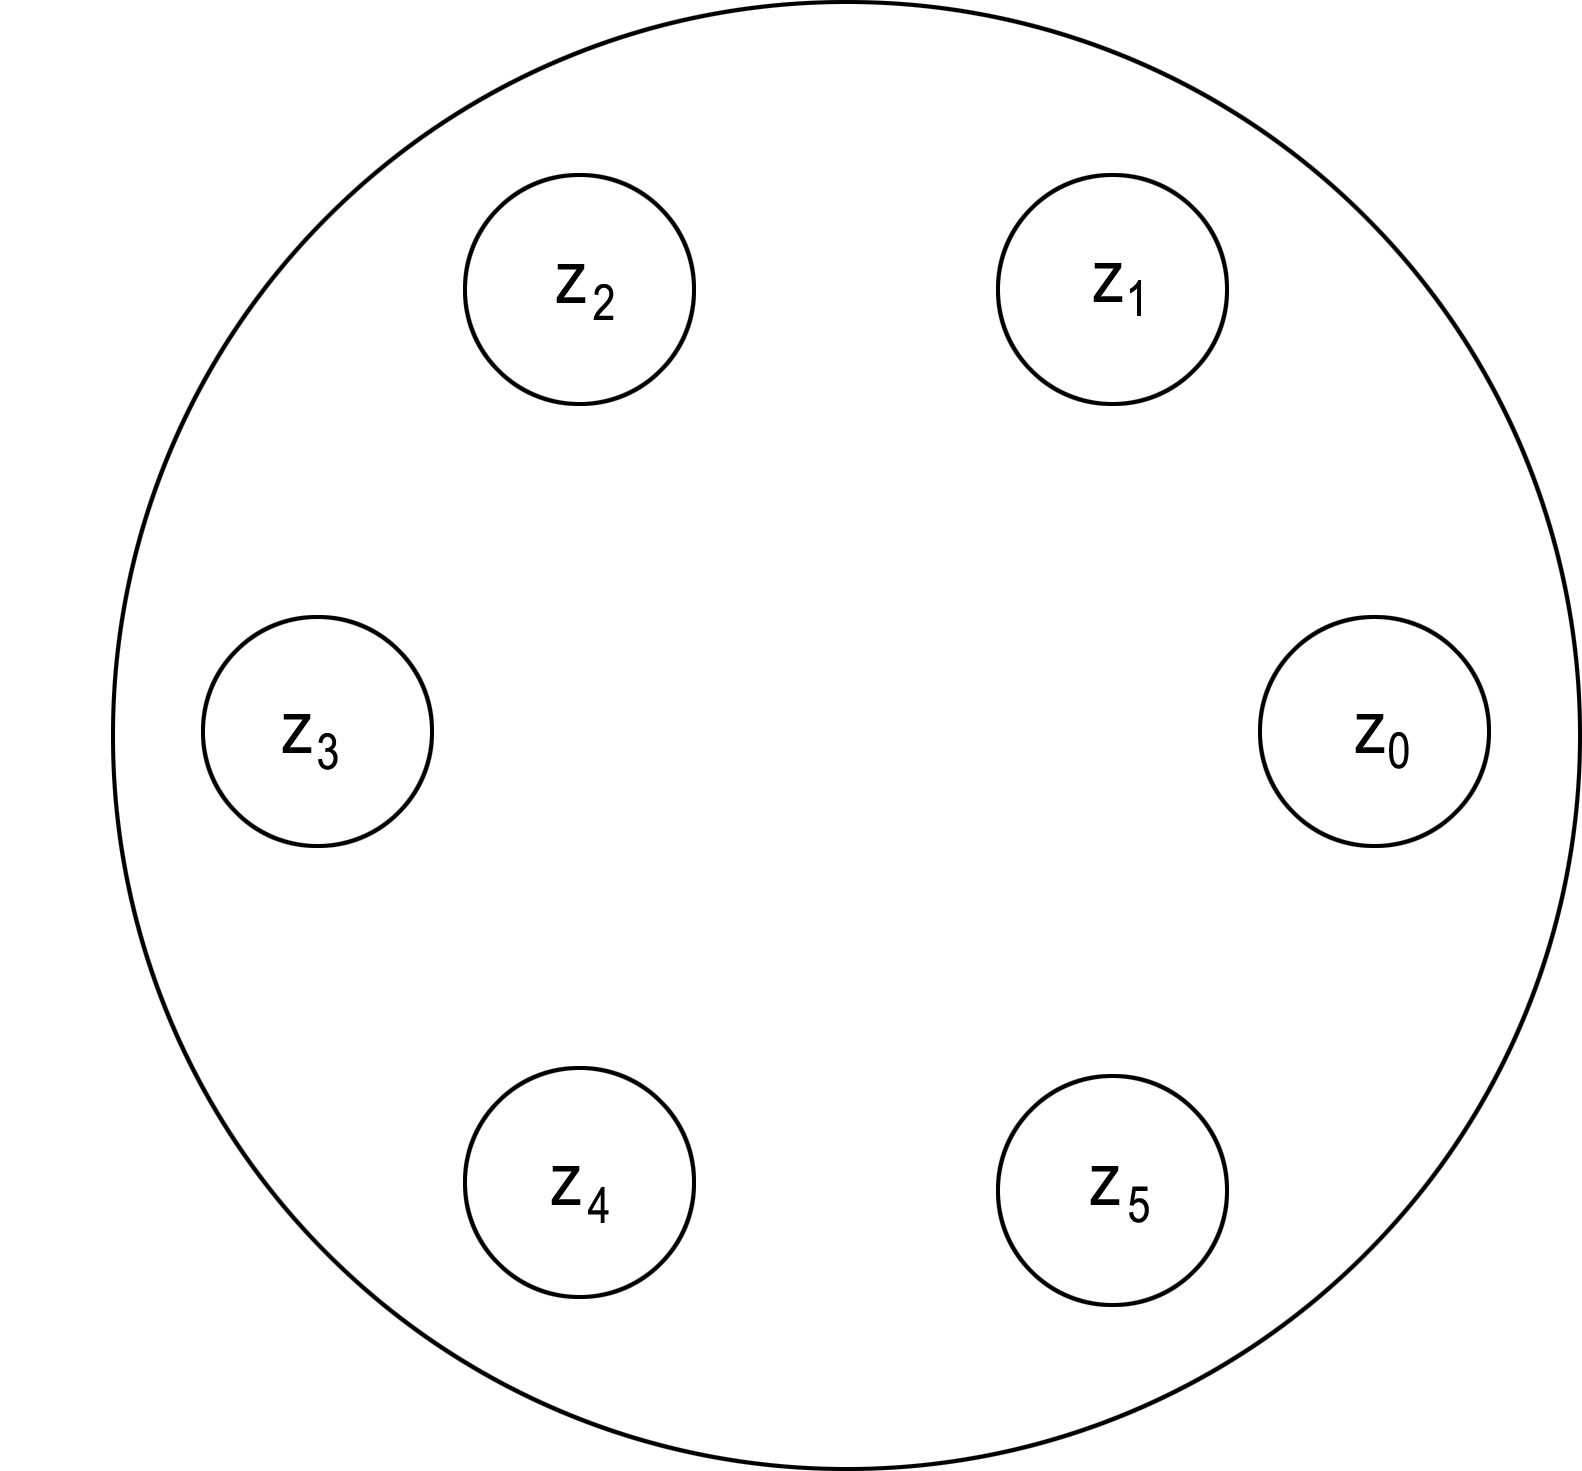
\includegraphics[width=0.4\textwidth]{pix/pants7.png}
\label{figure-originalhirsch}
\end{center}

  \vfill
  
}
  
 \frame
{
  \frametitle{Semi-simplicial realization of flat bundles}

Let $\G_{2,n} = (\mD^2, \mZ_n)$   denote the associated groupoid.

 \medskip
 
 $| \G_{2,n}| $ is the semi-simplicial space realizing the groupoid. 
 
 \medskip
 
 Then the classifying map factors:
 
 \medskip
 
$$ \mE_{n,k} \to | \G_{2,n}| \to B\G_2$$
 
 {\bf Corollary:} 
  $H^*(BSO_2 ; \mZ_n) \to H^*(B\G_2 ; \mZ_n) \to H^*(| \G_{2,n}| ; \mZ_n)$ 
  
  is injective for all $*$ and all $n \to \infty$.
  
  \vfill
  
}

\frame
{
  \frametitle{Construction of solenoids}

Choose   $n_1 < n_2 < \cdots $ tending to infinity   rapidly. Example: $n_k =      3^{k!}$
\medskip

Choose  $\epsilon_k \to 0$ rapidly, but slower than $1/n_k$. Example: $\epsilon_n = \epsilon_0 \cdot (3^n d_n)^{-1}$

\medskip
Restriction of  $\G_{2,n_1} = (\mD^2, \mZ_{n_1})$ to the invariant set

$$\cS_1 = \mD^2_{1,0} (z_{1,0},\epsilon_1) \cup  \mD^2_{1,1} (z_{1,1},\epsilon_1) \cup \cdots \cup  \mD^2_{n-1} (z_{1, n_1-1},\epsilon_1) $$
 is free, so we can repeat this construction of an action on $\cS_1$. 
 
\medskip


Choose  $z_{2,0} \in \mD^2_{1,0} (z_{1,0},\epsilon_1)$ which is not on center. 
\medskip

Repeat above construction for $\mZ_{n_2}$ on disks $\mD^2_{2,0} (z_{2,0},\epsilon_2)$. 
\medskip

There is one catch! Cannot just insert this action into $\G_{2,n_1}$. The plug will not be smooth.

\medskip

 Need to make deformation of action from identity on boundary of $V_1$ to rotation by $2\pi/n_2$ on boundary of $\mD^2_{2,0} (z_{2,0},\epsilon_2)$. 

  \vfill
  
}

\frame
{
  \frametitle{Picture of stage 1: $n_1 = 2$}
  
  \begin{center}
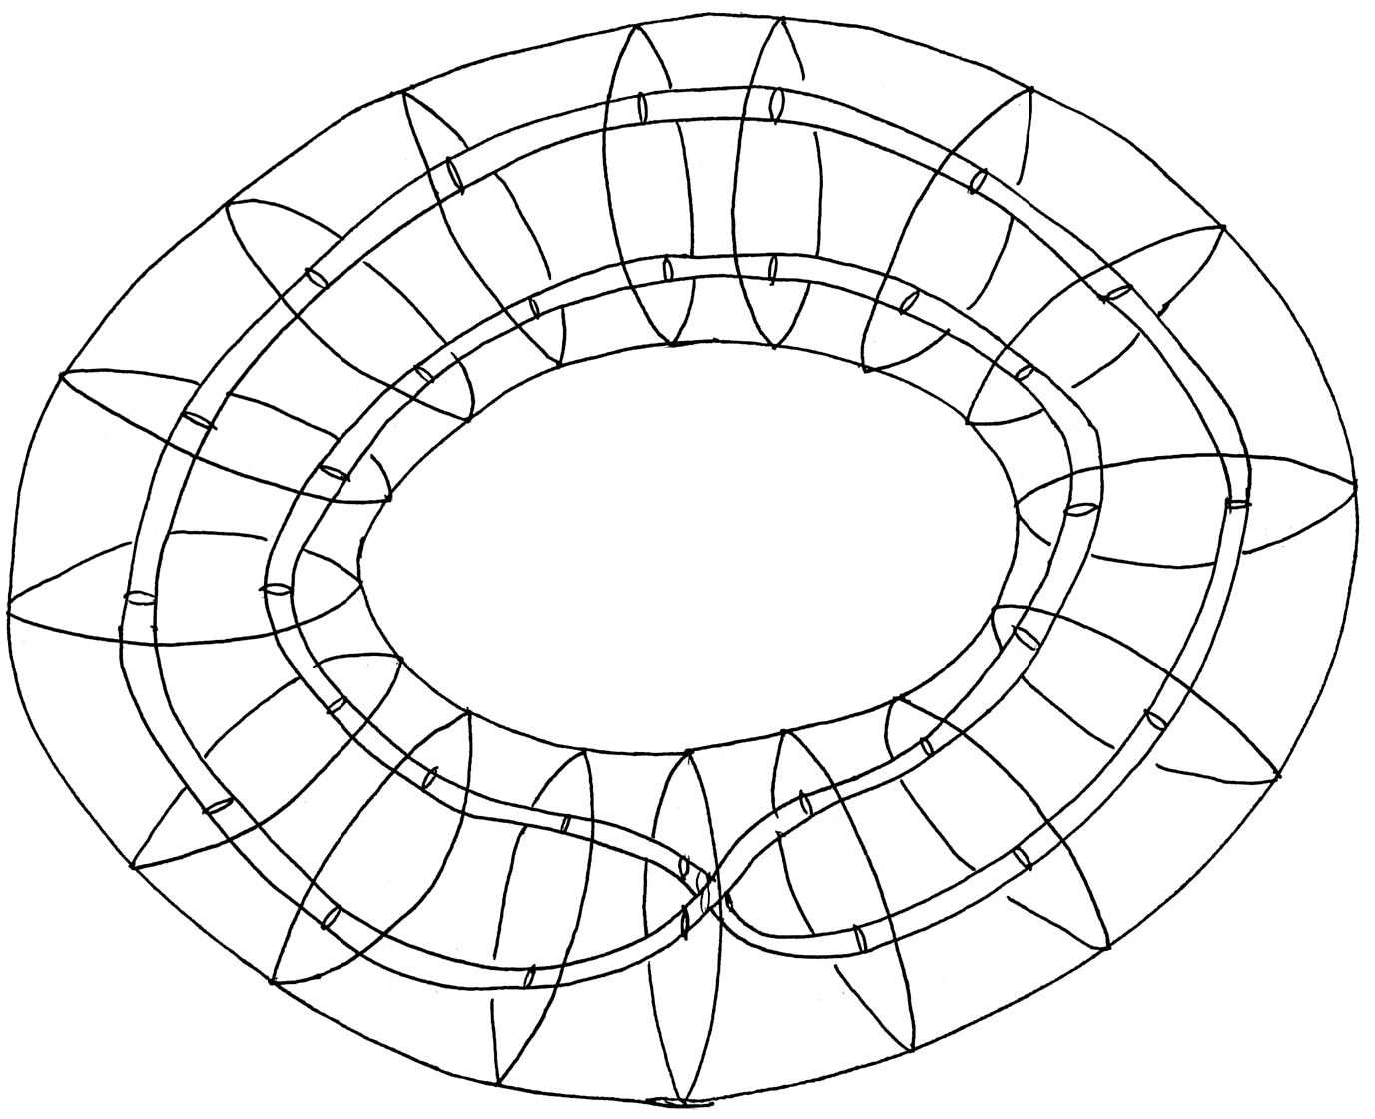
\includegraphics[width=0.6\textwidth]{pix/hirschplug.pdf}
% \caption{Original Hirsch construction illustrated}
\label{figure-originalhirsch2}
\end{center}


  \vfill
  
}
  
 
\frame
{
  \frametitle{Limit solenoid}
  
 Let $\G_{2,\infty}$ the smooth groupoid resulting from the limit of this construction. The action on $\mD^2$ is   distal!
 \medskip
 
 {\bf Proposition:} The dynamics of $\G_{2,\infty}$ contains a solenoidal minimal set
 $$\cS = \bigcap_{k=1}^{\infty} | \cS_k |$$
 
 \medskip
 
 
{\bf Proposition:} For every open neighborhood $\cS \subset U \subset |\G_{2,\infty}|$ there exists some $k \gg 0$ such that 
$|\cS_k| \subset U$

\medskip

{\bf Corollary:} 
For   $k \gg 0$ there is an inclusion
$|\G_{2,k}| \subset |\G_{2,\infty}|$.
 

 
 
  \vfill
  
}
  
   
\frame
{
  \frametitle{Homotopical consequences}
  
  Let $U$ be an open neighborhood, $\cS \subset U \subset | \G_{2,\infty}|$.
  
  \medskip
  
  {\bf Proposition:} 
  $H^*(BSO_2 ; \mZ) \to H^*(B\G_2 ; \mZ) \to H^*(U ; \mZ)$ is injective.
 
 \bigskip
 \pause
 
  {\bf Corollary:} The image of the classifying map 
  $U \to B\G_2$ cannot have finite type in all odd dimensions $> 4$.
 
 \bigskip
 \pause
 
 One obtains framed foliations by considering the frame bundle $\widehat{U} \to U$ of the normal bundle on $U$. 
 
 \medskip
 
 The foliation $\F$ on $U$ lifts to a foliation $\widehat{\F}$ on $\widehat{U}$. 
 
 \medskip
 
 By finite-type considerations, we obtain
 
 \medskip
 
 {\bf Theorem:} The image of the classifying map $\widehat{U} \to F\G_q$ cannot have finite type in all odd dimensions $> 4$.

 
 
  \vfill
  
}
  
     
\frame
{
  \frametitle{Chern-Simons invariants}
  
{\bf Theorem:} 
 The Chern-Simons invariants in $H^{2*-1}(B\G_2 ; \mR/\mZ)$ are non-trivial on the image of  $| \G_{2,\infty}| \to B\G_q$   in all odd dimensions $> 4$.

\bigskip
\pause
 
 {\bf Remark 1:} Apparently, the transgression classes of the Pontrjagin classes  $H^{4*}(BSO_q ; \mR)$ do not 
 depend on dynamics in the same way as before. 
 
 \bigskip
\pause

 
  {\bf Remark 2:}  The above construction admits many generalizations to embedded braid diagrams. Unclear what cohomology theories will be needed to detect them.
 
  \vfill
  
}
  


 
\end{document}
       
 